\section{Pruebas.}
\subsection{Pruebas de usabilidad.}

La evaluación de usabilidad del launcher se realizó con estudiantes universitarios, grupo objetivo de la aplicación. Los participantes, en su mayoría jóvenes adultos entre 22 y 25 años que usan su smartphone regularmente, reflejan el perfil típico de usuarios que buscan mejorar su concentración y productividad. La mayoría manifestó ser consciente del tiempo excesivo que pasa en su smartphone, especialmente en momentos inapropiados como durante actividades académicas o de descanso, y expresó interés en herramientas que les ayuden a regular este uso.

Cabe destacar que el número de encuestados fue reducido debido a las particularidades técnicas y éticas del proyecto. Dado que se trata de una aplicación para Android que se debe instalar, no es posible su despliegue en un entorno web ni su distribución pública, ya que su instalación requiere permisos especiales relacionados con acceso a información del sistema operativo y el monitoreo del tiempo de uso de las aplicaciones, aspectos que son sensibles en términos de privacidad.

Por estas razones, se decidió aplicar la encuesta únicamente a un grupo selecto de usuarios que aceptaron instalar la aplicación en sus dispositivos personales y participar bajo las condiciones previamente informadas, garantizando así un entorno de prueba controlado, seguro y éticamente responsable.

\subsubsection{Resultados de la encuesta.}

La Figura \ref{fig:interfaz_intuitiva} muestra que la mayoría de los participantes considera que el launcher es intuitivo y fácil de usar. El 71,4\% de los participantes calificó con la puntuación máxima (5) la intuición de la interfaz del launcher, mientras que el 28,6\% le otorgó una calificación de 4.

\begin{figure}[h]
  \caption{Primera prueba de usabilidad.}
  \label{fig:interfaz_intuitiva}
  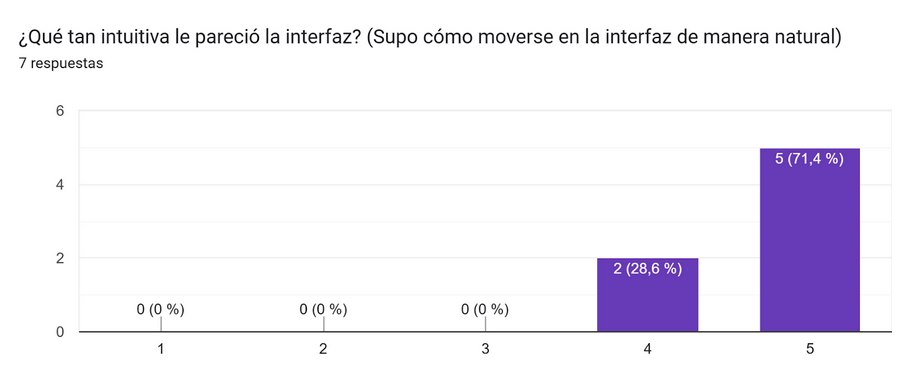
\includegraphics[width=\textwidth]{Figuras/interfaz_intuitiva.png}
  \centering
\end{figure}

En relación con la apariencia de la aplicación, los resultados presentes en la Figura \ref{fig:interfaz_agradable} reflejan una alta aceptación del diseño minimalista, funcional y centrado en la productividad por parte de los usuarios. El 71,4\% de los encuestados calificó el diseño de la interfaz con la puntuación máxima (5), mientras que el 28,6\% otorgó una calificación de 4.

\begin{figure}[h]
  \caption{Segunda prueba de usabilidad.}
  \label{fig:interfaz_agradable}
  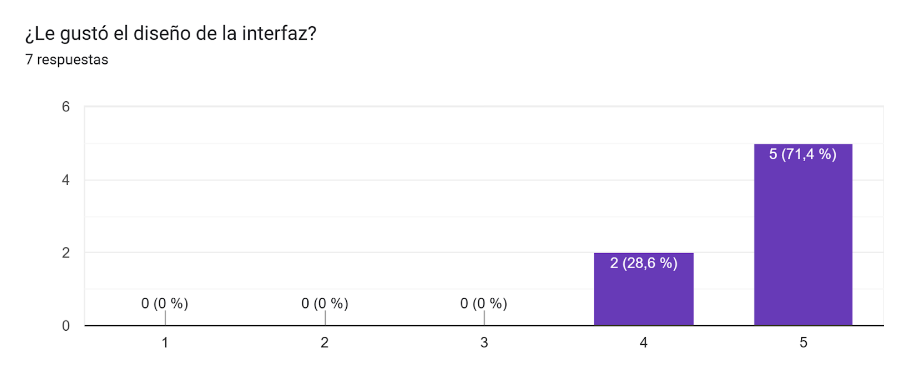
\includegraphics[width=\textwidth]{Figuras/interfaz_agradable.png}
  \centering
\end{figure}

Los resultados de la tercera prueba de usabilidad, mostrados en la Figura \ref{fig:mejores_caracteristicas}, indican que el diseño minimalista fue identificado como la característica más útil del launcher por el 100\% de los participantes. En segundo lugar, se destacan la gestión de tareas y hábitos (71,4\%) y el límite de uso de aplicaciones (71,4\%), dos de las principales funcionalidades del launcher. 

\begin{figure}[h]
  \caption{Tercera prueba de usabilidad.}
  \label{fig:mejores_caracteristicas}
  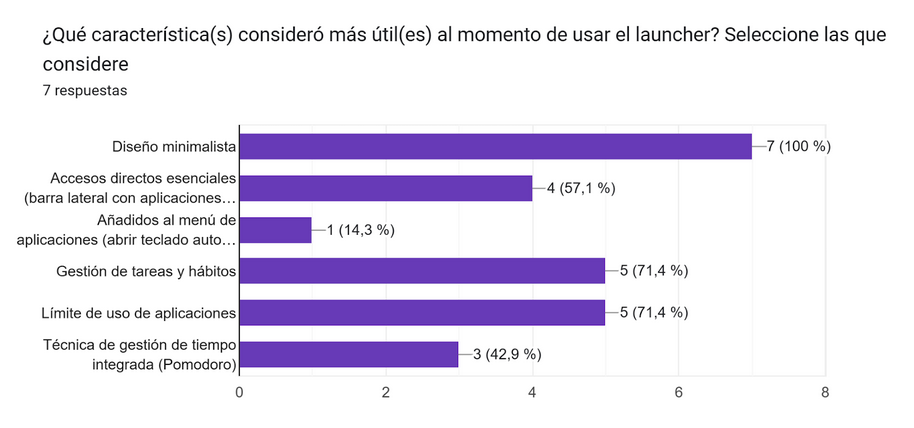
\includegraphics[width=\textwidth]{Figuras/mejores_caracteristicas.png}
  \centering
\end{figure}